\excnt=1
\chapter{The argument structure of modals}
\label{chap:arg}

\chapterprecishere{Are modals really raising predicates? Are they at least
  sometimes control predicates? If they are ``raising'' predicates, is that
  syntactic raising or some kind of ``semantic'' raising?}

\minitoc

\section{Raising vs. Control}
\label{sec:raising-control}

In lieu of lecture notes, a part of a handout from a class on ``Morphology,
syntax, and semantics of modals'' taught by Kai von Fintel and Sabine at the 2009
LSA Summer Institute at the University of California at Berkeley.

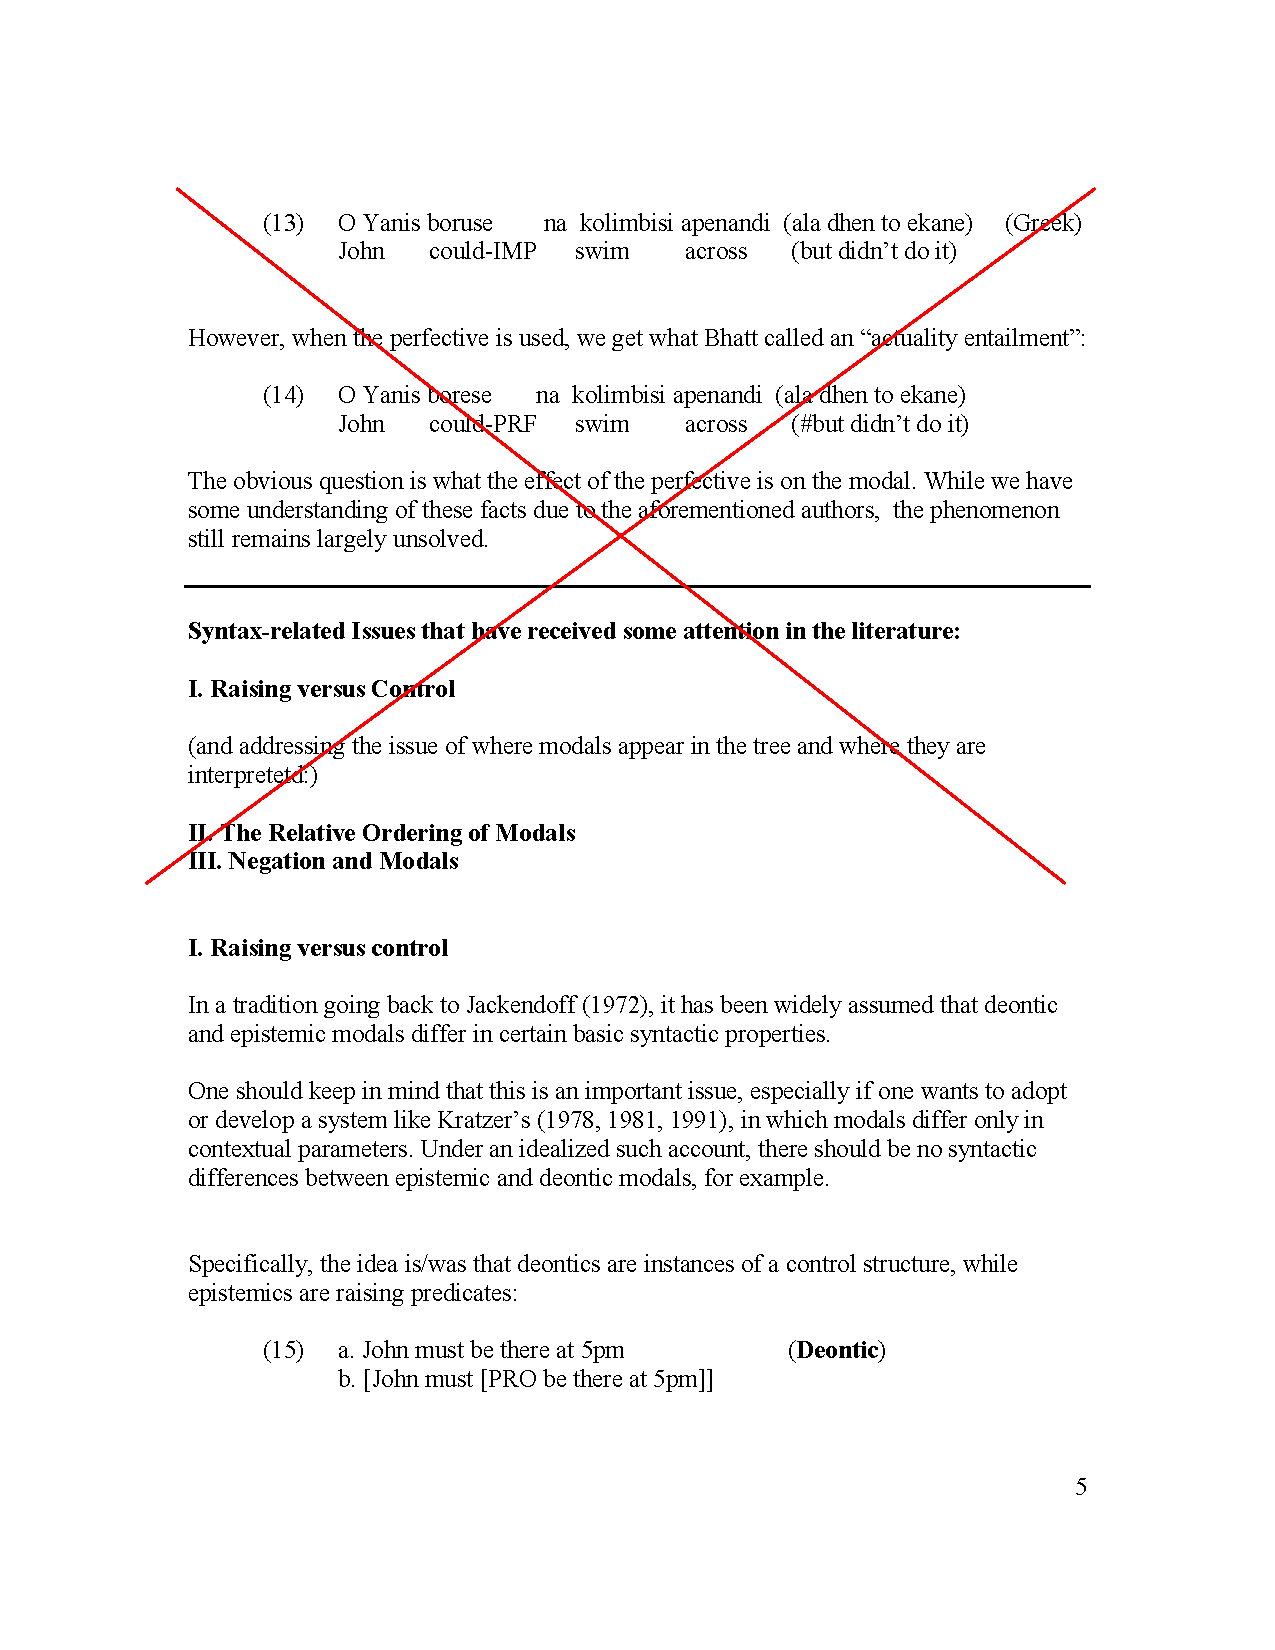
\includepdf[pages=-,frame=true]{fintel-iatridou-2009-lsa-modals-raising-control.pdf}

\newpage
\section{``Semantic'' Raising}
\label{sec:semantic-raising}

Unedited lecture notes from 2002.

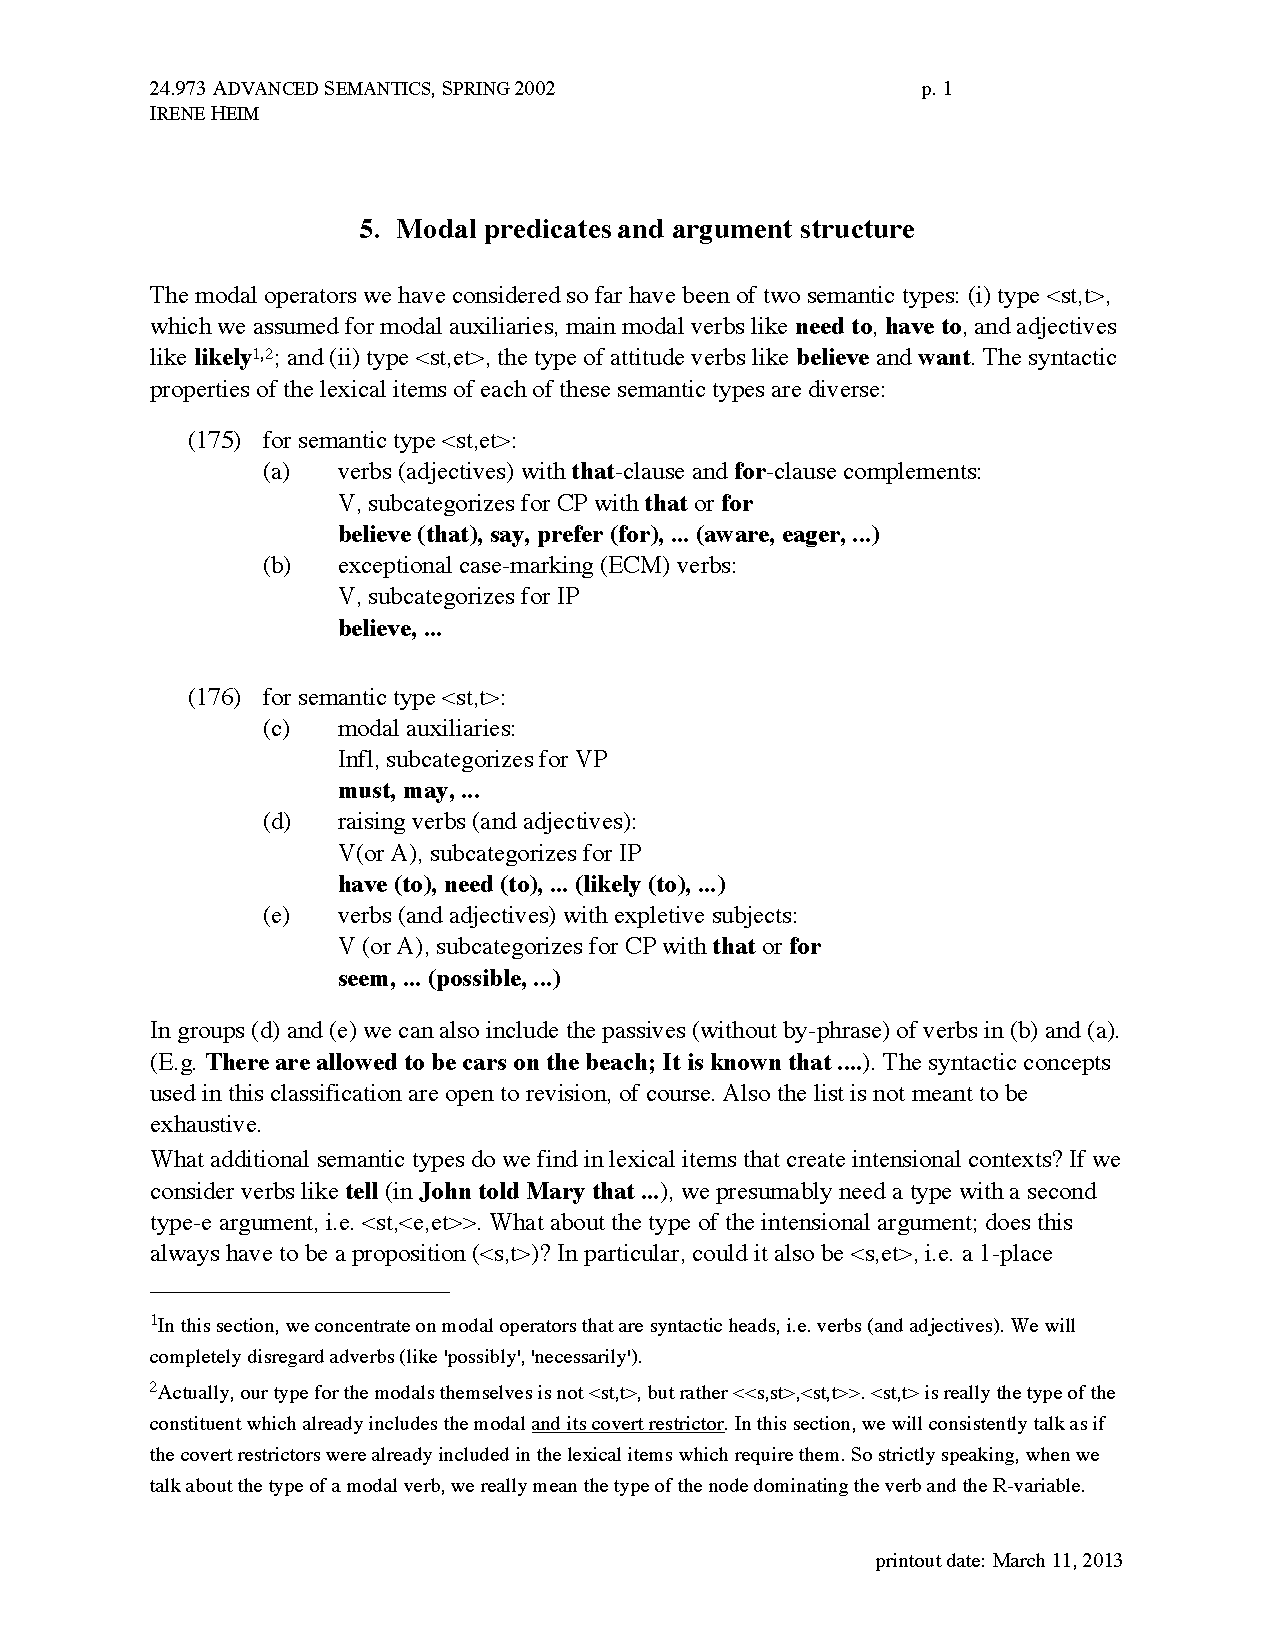
\includepdf[pages=-,frame=true]{lectures_notes_control_raising_2013.pdf}





